% BASIC SETTINGS
\documentclass[a4paper,12pt]{article} % Set paper size and document type
\usepackage{lmodern} % Use a slightly nicer looking font
\usepackage{url} % Proper formatting for URLs
\usepackage{graphicx} % Handle inclusion of non-PDF graphics
\usepackage{subfig} % Allow sub-figures inside a figure
\usepackage{enumitem} % Allow lists to pick up numbering where the last list left off

% Change margins - default margins are too broad
\usepackage[margin=20mm]{geometry}
\usepackage{amsmath}

% SOURCE CODE LISTING SETTINGS 
% https://en.wikibooks.org/wiki/LaTeX/Source_Code_Listings
\usepackage{listings}
\usepackage{color}

% Color definitions for source code listings
\definecolor{mygreen}{rgb}{0,0.6,0}
\definecolor{mygray}{rgb}{0.5,0.5,0.5}
\definecolor{mymauve}{rgb}{0.58,0,0.82}

\definecolor{codegreen}{rgb}{0,0.6,0}
\definecolor{codegray}{rgb}{0.5,0.5,0.5}
\definecolor{codepurple}{rgb}{0.58,0,0.82}
\definecolor{backcolour}{rgb}{0.95,0.95,0.92}

\lstdefinestyle{mystyle}{
    backgroundcolor=\color{backcolour},   
    commentstyle=\color{codegreen},
    keywordstyle=\color{magenta},
    numberstyle=\tiny\color{codegray},
    stringstyle=\color{codepurple},
    basicstyle=\ttfamily\footnotesize,
    breakatwhitespace=false,         
    breaklines=true,                 
    captionpos=b,                    
    keepspaces=true,                 
    numbers=left,                    
    numbersep=5pt,                  
    showspaces=false,                
    showstringspaces=false,
    showtabs=false,                  
    tabsize=2
}

\lstset{style=mystyle}

% Set document title and author
\title{\LaTeX \space{} Example \#1}
\author{Jeremy Pedersen}
\date{2023-01-03} % If date is left blank, it will be hidden

% Document body
\begin{document}

\maketitle % Insert the title, author, and date

\section{First section} %  Create a section

We can use the listing package to place source code into our documents from a file:

% Include code from a file with filename indicated
\vspace{5mm}
\lstinputlisting[language=Python, caption=Rangoli generator]{test_code.py}
\vspace{5mm}

\noindent
Or we can quote a range of line numbers from the file (lines 19 and 20, for example):

% Include only specific lines from a file
\vspace{5mm}
\lstinputlisting[language=Python, firstline=19, lastline=20, caption=Rangoli generator specific part]{test_code.py}
\vspace{5mm}

% Forces content onto the next page, useful for documents which should look nice when printed out
\clearpage

\noindent
We can also place code directly into latex without importing it from a file:

% Include code inline
\vspace{5mm}
\begin{lstlisting}[language=Python, caption=Python example]
print("Hi, I'm Python 3!")
\end{lstlisting}
\vspace{5mm}

\subsection{First subsection} % Create a subsection

We can create and format mathematical expressions like so:

% Format a mathematical expression
\begin{align}
\label{eqn:eqlabel}
\begin{split}
x' = x \cdot s \cos\left(\theta\right) - y \cdot s \sin\left(\theta\right) + t_x
\\
y' = x \cdot s \sin\left(\theta\right) + y \cdot s \cos\left(\theta\right) + t_y
\end{split}
\end{align}

\noindent
We can also make a nice list:

% Make a list
\vspace{2mm}
\begin{enumerate}
\item I am the first thing in the list
\item I am the second thing in the list
\end{enumerate}
\vspace{2mm}

Reference the previous equation with (\ref{eqn:eqlabel}).

\noindent
We can inline mathematical expressions such as this one "$4 \sigma_0$" using the "\$" sign. We can make mathematical expressions that occupy their own line, like this: 
\[
u = \left(x - x_0\right) {1 \over 4 \sigma_0} \cos\left(\theta_0\right) - \left(y - y_0\right) {1 \over 4 \sigma_0} \sin\left(\theta_0\right) + 4 = \left(0 - 16\right) \frac{1}{4} - 0 + 4
\]

\subsection{Second subsection}

We can also make tables and charts using the array type like so.

Let $\theta_0$ be a fixed, nonnegative real number smaller than $2\pi$, let $\phi$ be a function of the real variable $\theta \in [0, 2\pi)$ defined as follows:
% Make an array or table
\vspace{2mm}
\[ \phi \left(\theta\right) = \left\{ 
\begin{array}{l l}
\theta_0 + \theta & \, \textrm{if} \, \theta_0 + \theta \in [0,2 \pi)\\ 
\theta_0 + \theta + 2 \pi & \, \textrm{if} \, \ \theta_0 + \theta < 0\\
\theta_0 + \theta - 2 \pi & \, \textrm{if} \, \theta_0 + \theta \ge 2 \pi\\
\end{array} \right.
\] 
\vspace{2mm}

\noindent
I can start an enumerated list of items here...

\vspace{5mm}
\begin{enumerate}
\item One thing
\item Another thing
\end{enumerate}
\vspace{5mm}

\noindent
And then...

\section{Second section}

...I can continue it here!

\vspace{5mm}
\begin{enumerate}[resume]
\item Yet more stuff
\item Some other things
\end{enumerate}
\vspace{5mm}

Inserting figures is also relatively easy to do: 

\vspace{5mm}
% Insert a figure with an image
\begin{figure}[!ht]
  \centering
  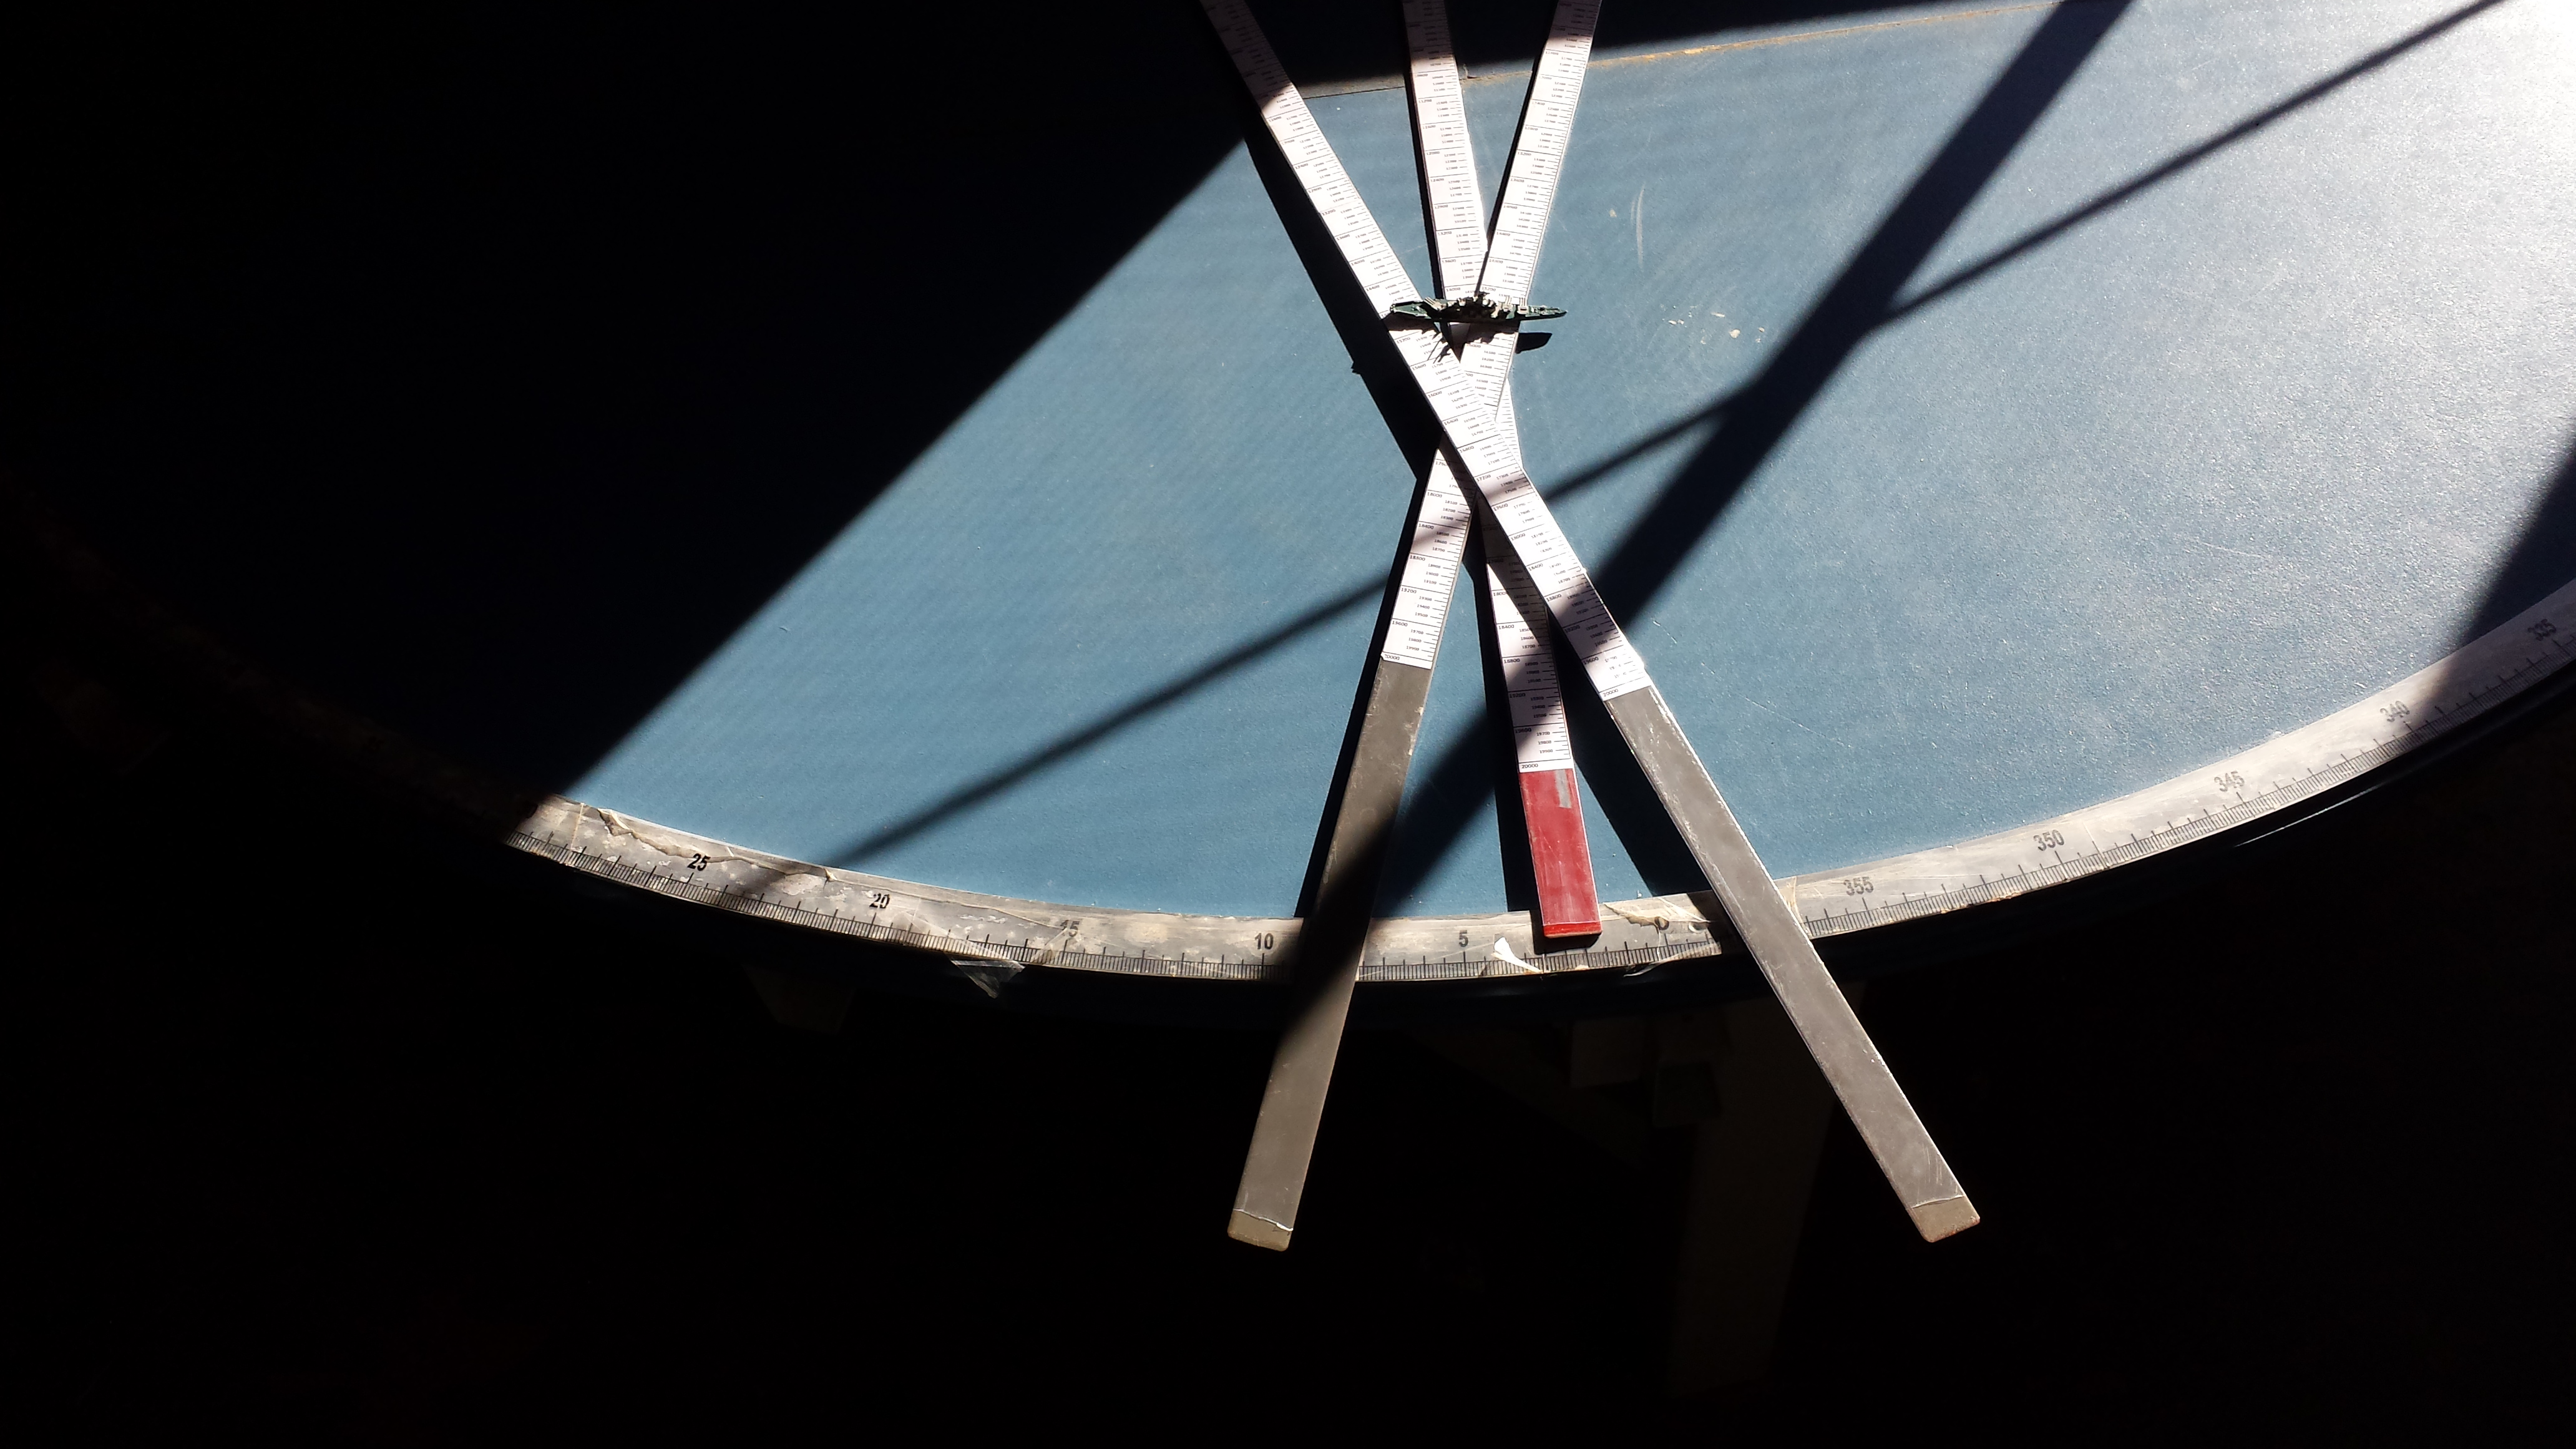
\includegraphics[width=0.5\textwidth]{test_image.jpg}
  \caption{I can embed images too}
\end{figure}

\noindent
We can make a table with centered elements:

\vspace{5mm}
\[ \left[ \begin{array}{c c c}
1.1754 & -0.8334 & 193.4191\\
0.2062 & 1.0380 & -141.0333\\
-0.0008 & 0.0007 & 1.0000\\
\end{array}
\right] \]
\vspace{5mm}

\noindent
There you go! That should be enough to get you started on \LaTeX!

\lstlistoflistings

\end{document}
